\section{Trực quan hóa dữ liệu}

% ================= SUBSECTION 1 =================
\subsection{Tổng quan bộ dữ liệu}
% Gom 2 hình tổng quan Dashboard, biểu đồ tròn và phân bố pH vào chung 1 mục

\begin{figure}[H]
    \centering
    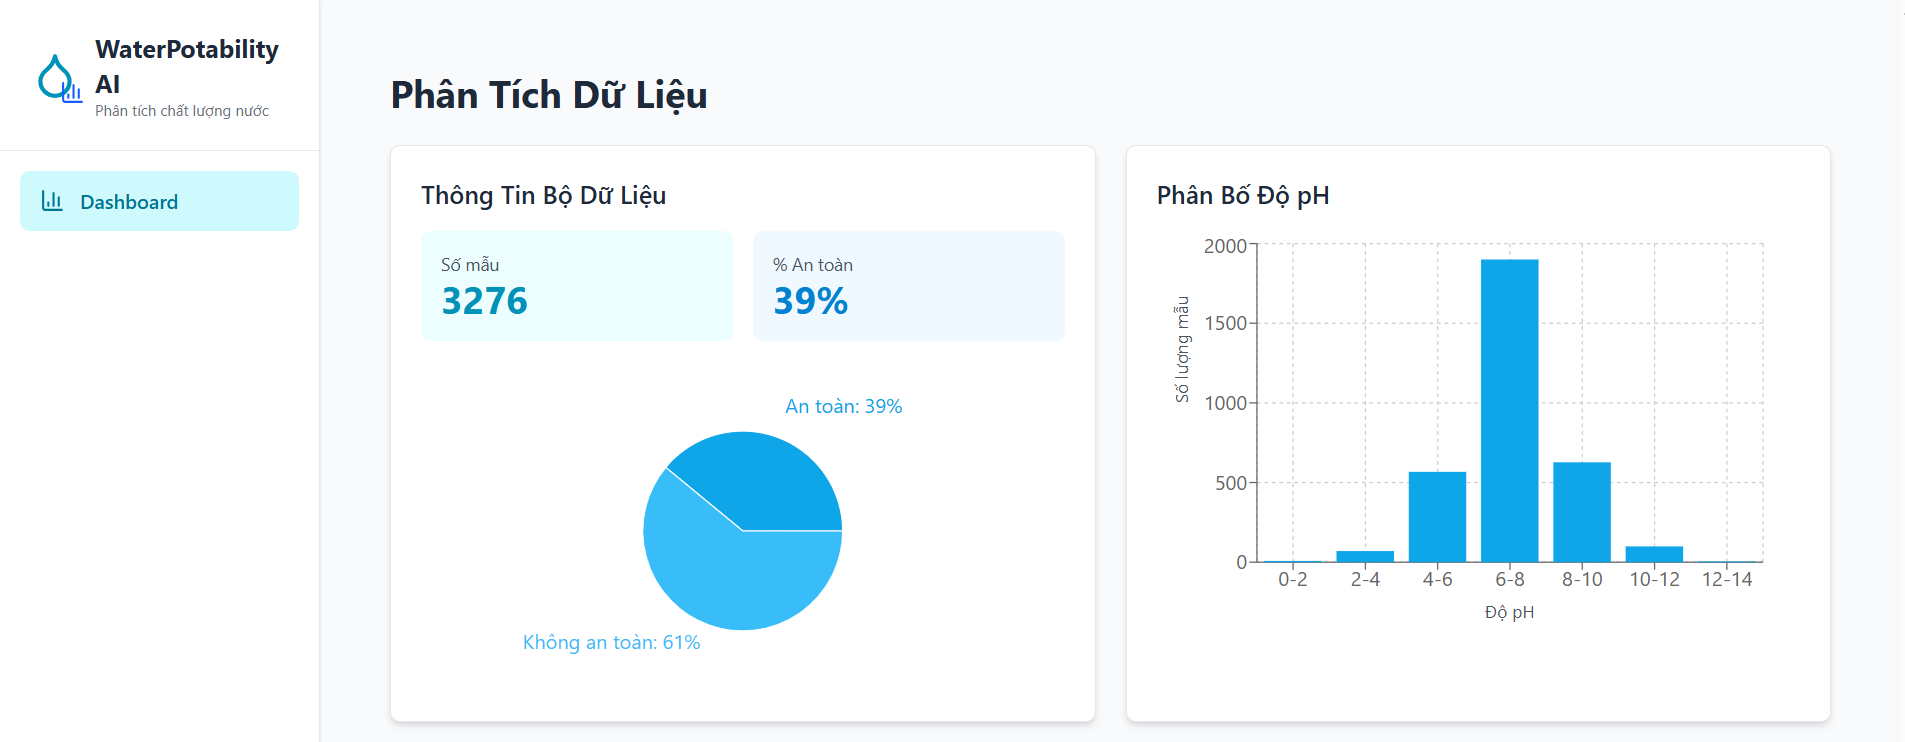
\includegraphics[width=0.9\textwidth]{IMAGE-PENTAHO/pentaho-1.png}
    \caption{Giao diện tổng quan phần Phân tích dữ liệu hiển thị thông tin bộ dữ liệu, biểu đồ tròn tỷ lệ an toàn (được làm nổi bật phần trăm) và biểu đồ cột biểu diễn phân bố độ pH.}
    \label{fig:pentaho_1}
\end{figure}

\begin{figure}[H]
    \centering
    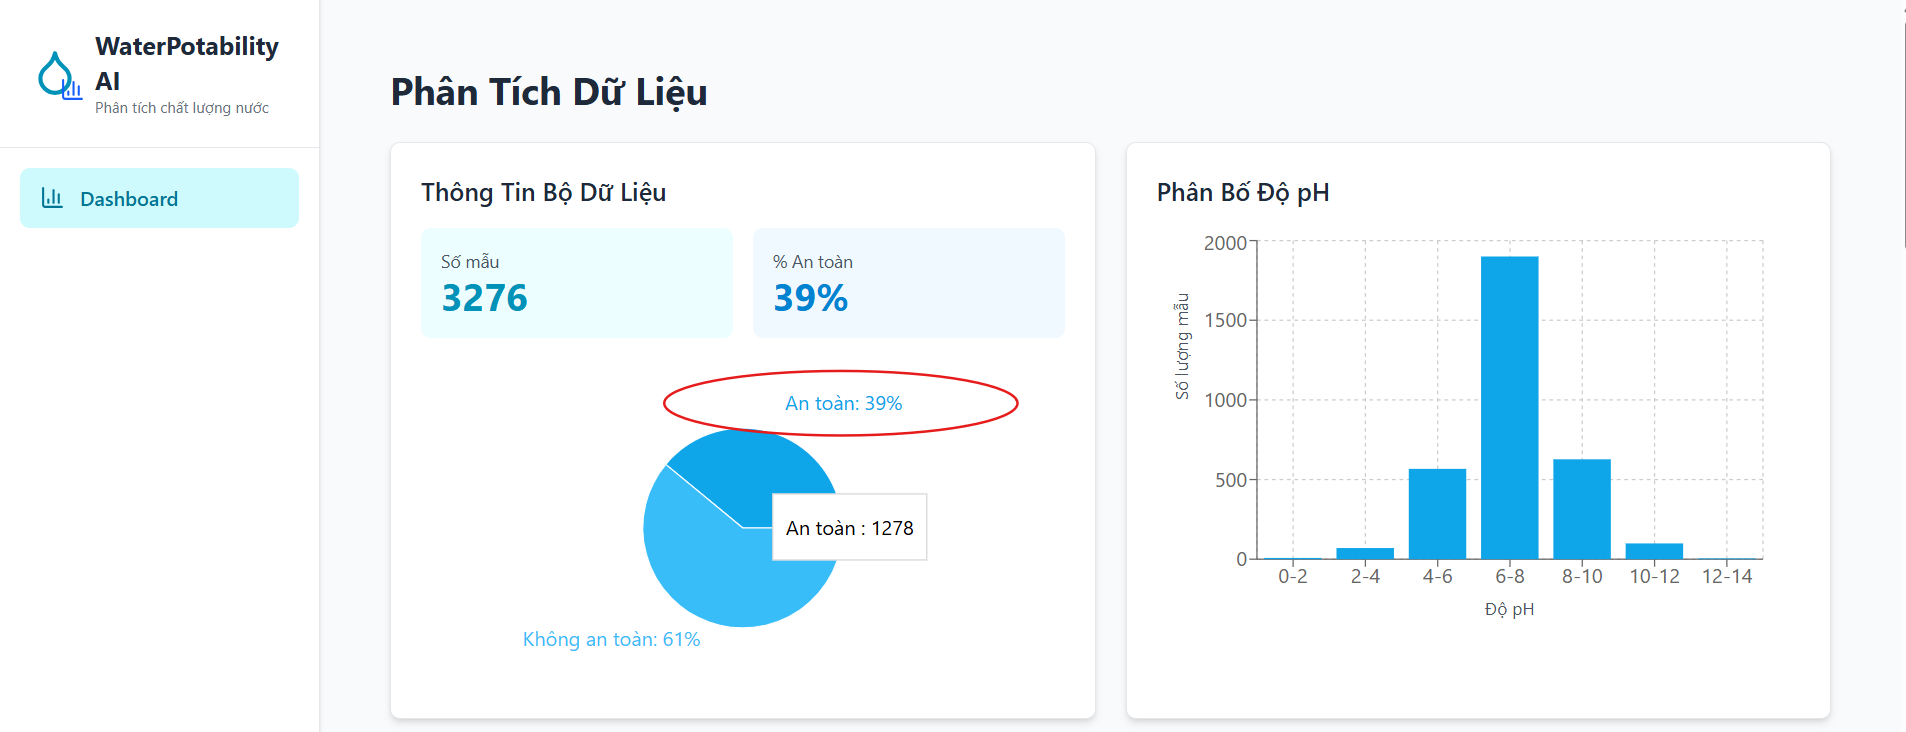
\includegraphics[width=0.9\textwidth]{IMAGE-PENTAHO/pentaho-6.png}
    \caption{Giao diện tổng quan Dashboard thể hiện chi tiết số liệu của bộ dữ liệu gốc bao gồm tổng số mẫu, tỷ lệ phần trăm mẫu nước an toàn/không an toàn và phân bố dữ liệu theo độ pH.}
    \label{fig:pentaho_6}
\end{figure}

% ================= SUBSECTION 2 =================
\subsection{Phân tích phân bố đặc trưng và Tương quan dữ liệu}
% Gom biểu đồ phân bố tứ phân vị (Độ cứng) và Ma trận tương quan Pearson

\begin{figure}[H]
    \centering
    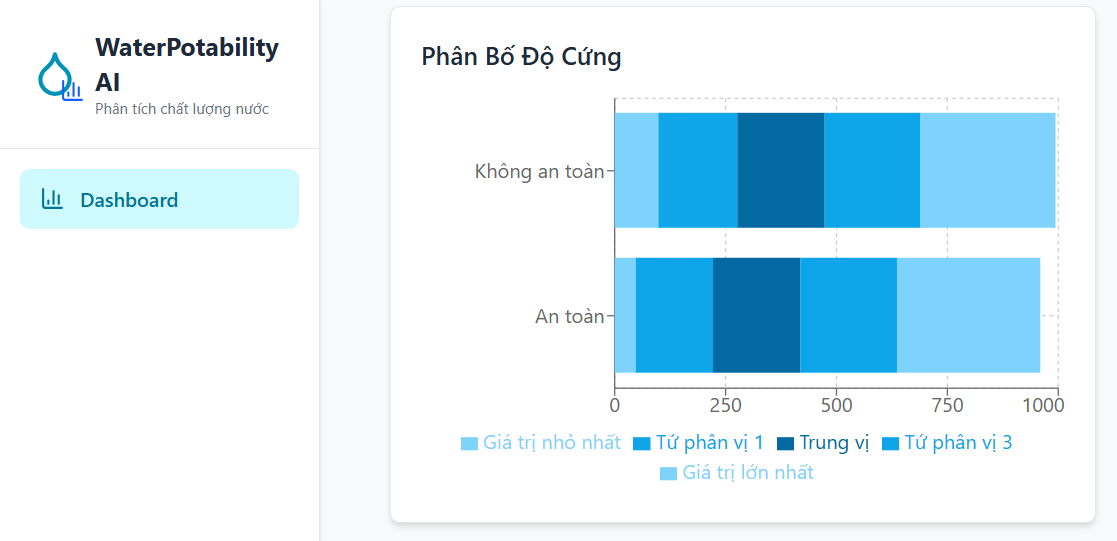
\includegraphics[width=0.9\textwidth]{IMAGE-PENTAHO/phân-bổ-độ-cứng.png}
    \caption{Giao diện trực quan hóa dữ liệu hiển thị biểu đồ phân bố độ cứng (kèm chú giải chi tiết các tứ phân vị, giá trị lớn nhất/nhỏ nhất).}
    \label{fig:phan_bo_do_cung}
\end{figure}

\begin{figure}[H]
    \centering
    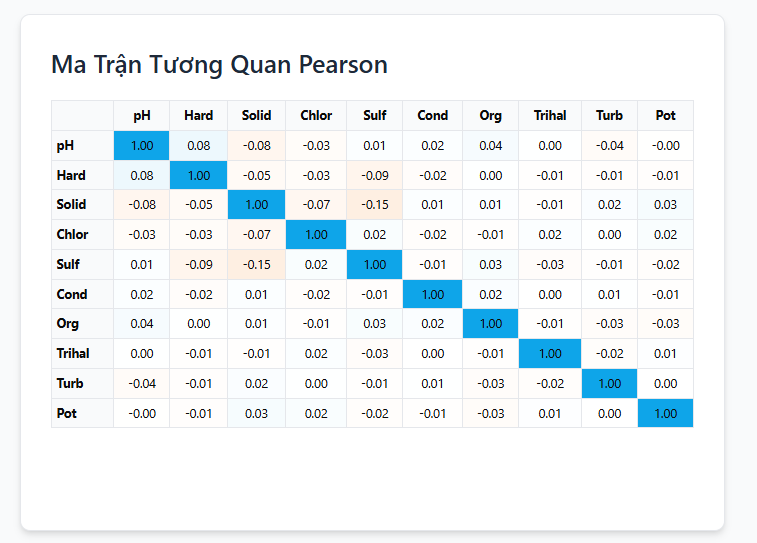
\includegraphics[width=0.9\textwidth]{IMAGE-PENTAHO/pearson.png}
    \caption{Ma trận tương quan Pearson giữa các chỉ số.}
    \label{fig:pearson_matrix}
\end{figure}

% ================= SUBSECTION 3 =================
\subsection{Phân tích mối quan hệ đa biến}
% Gom các biểu đồ phân tán (Scatter plot) và so sánh trung bình giữa 2 nhãn An toàn/Không an toàn

\begin{figure}[H]
    \centering
    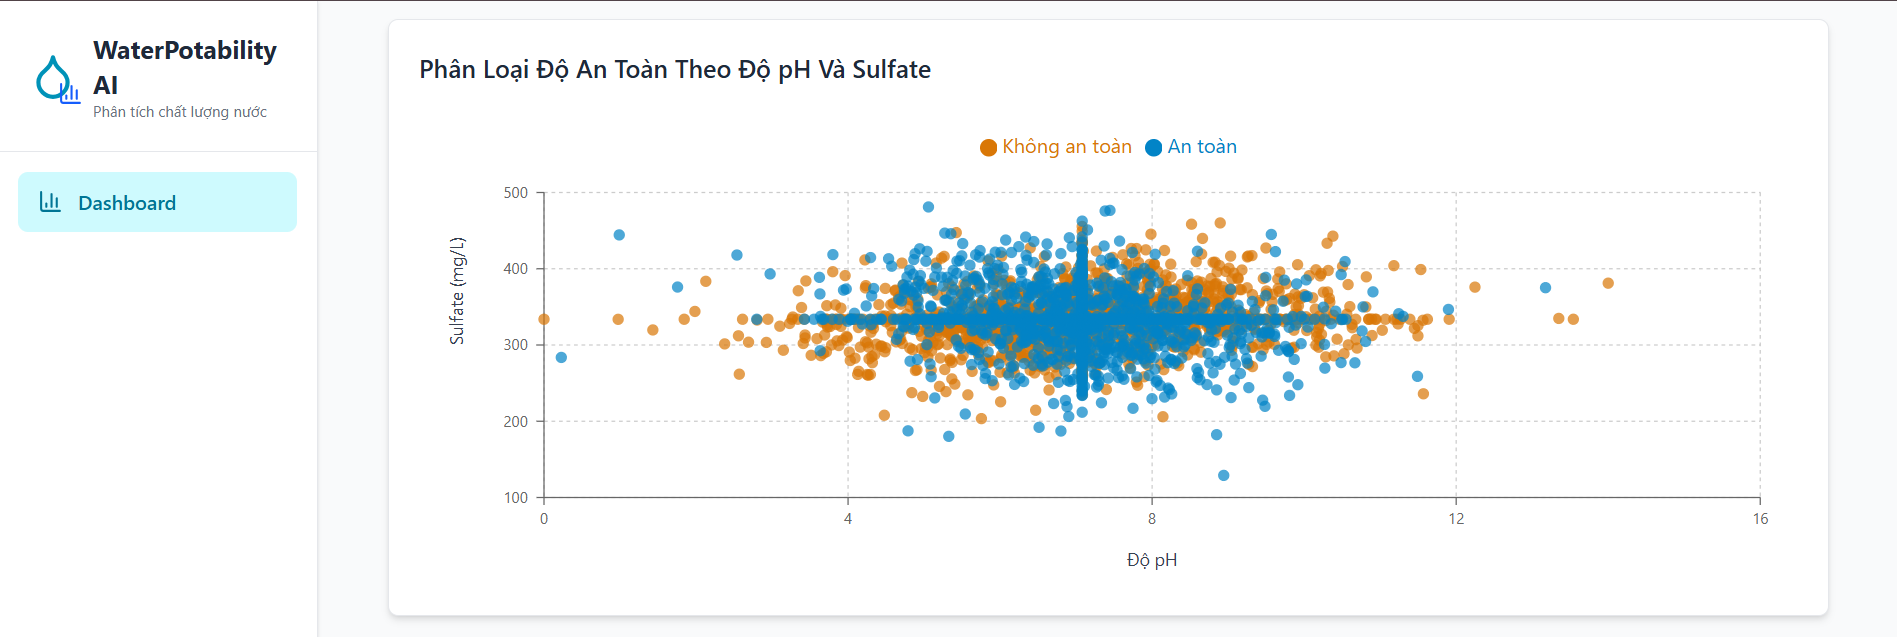
\includegraphics[width=0.9\textwidth]{IMAGE-PENTAHO/phân-loại-an-toàn.png}
    \caption{Biểu đồ phân tán (Scatter plot) thể hiện mối quan hệ và sự phân loại độ an toàn của nguồn nước dựa trên hai đặc trưng: độ pH và Sulfate.}
    \label{fig:phan_loai_an_toan}
\end{figure}

\begin{figure}[H]
    \centering
    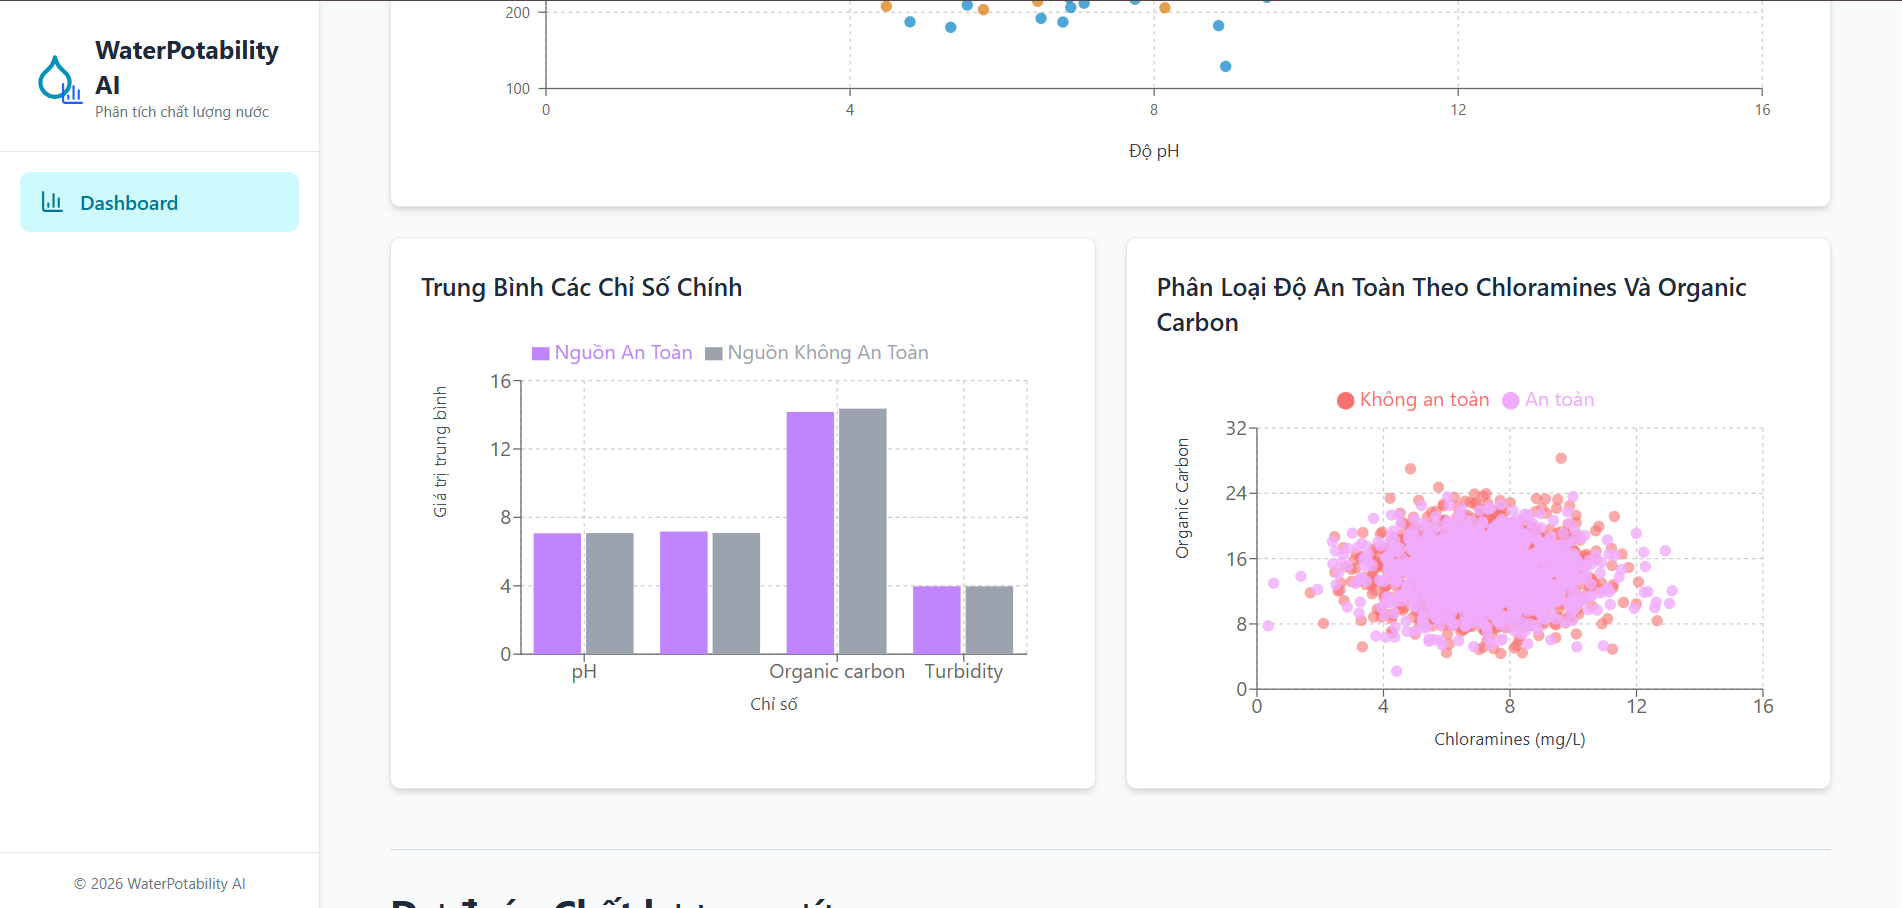
\includegraphics[width=0.9\textwidth]{IMAGE-PENTAHO/pentaho-4.png}
    \caption{Giao diện so sánh giá trị trung bình của các chỉ số chính (pH, Organic carbon, Turbidity) giữa hai nhóm an toàn/không an toàn và biểu đồ phân loại theo Chloramines và Organic Carbon.}
    \label{fig:pentaho_4}
\end{figure}

% ================= SUBSECTION 4 =================
\subsection{Giao diện dự đoán và Đánh giá mô hình}
% Tách riêng phần Demo giao diện dự đoán và các chỉ số (Accuracy, F1,...)

\begin{figure}[H]
    \centering
    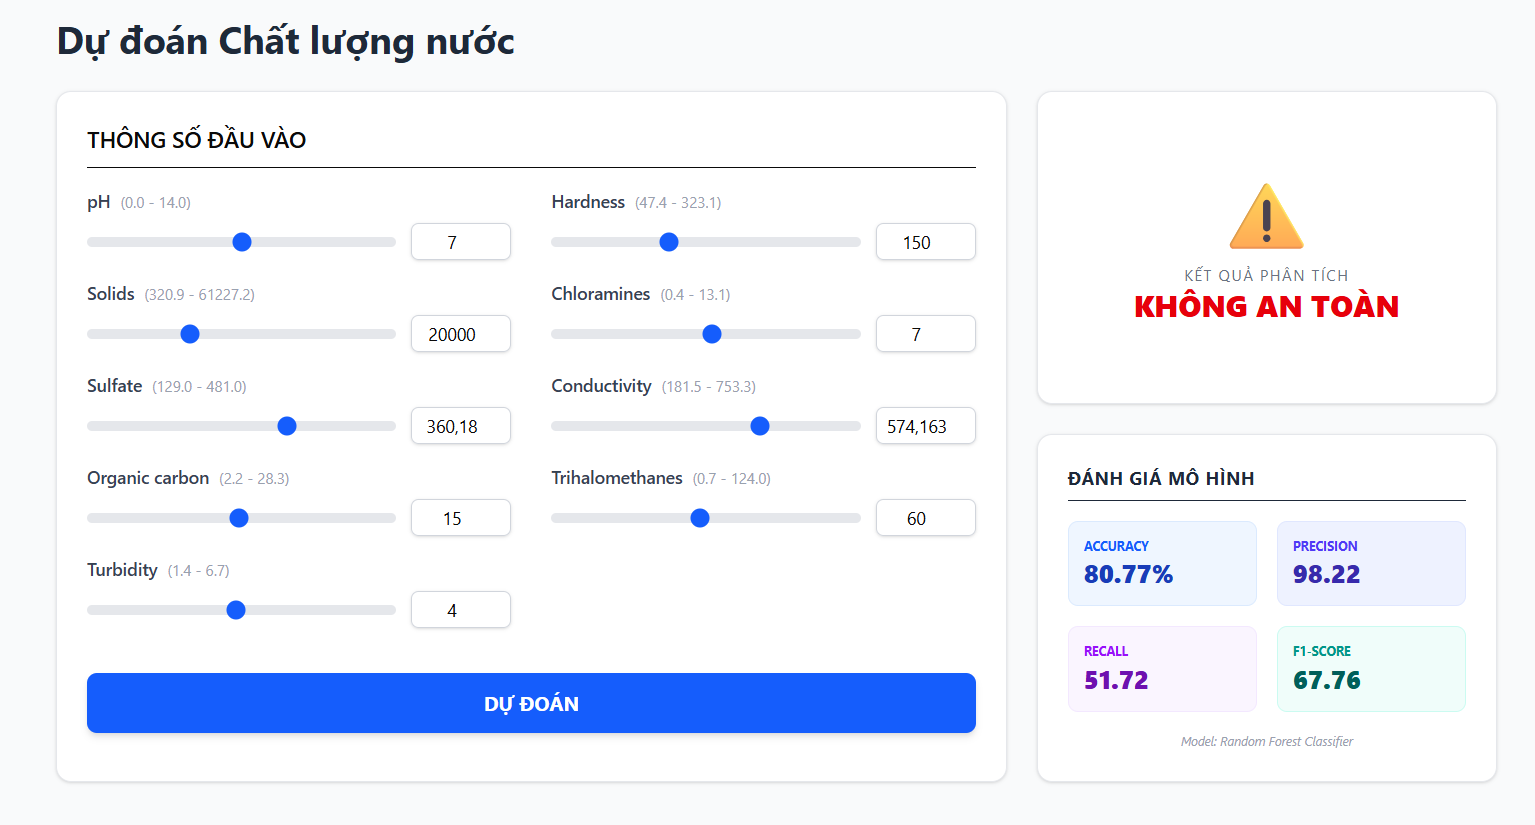
\includegraphics[width=0.9\textwidth]{IMAGE-PENTAHO/pentaho-5.png}
    \caption{Giao diện Dự đoán chất lượng nước cho phép người dùng tùy chỉnh các thông số đầu vào, hiển thị kết quả phân tích trực quan và các chỉ số đánh giá hiệu suất của mô hình (Accuracy, Precision, Recall, F1-Score).}
    \label{fig:pentaho_5}
\end{figure}